\chapter{Regression \label{chapter:regression}}

Classification is a form of supervised learning in which the outcome is a category. \textbf{Regression}\index{regression} is another form of supervised learning in which the outcome is a numeric value. For example, it may be a lab value, physical characteristic (height, weight, etc.), or numeric measurement (e.g. oxygen saturation).

%%%%%%%%%%%%%%%%%%%%%%%%%%%%%%%%%%%%%%%%%%%%%%%%%%%%%%%%%%%%%%%%%%%%%%%%%%%%%%%%%%%%%%

\section{Visualizing the Regression Problem \label{section:visualizingreg}}

Let's consider the same setup from Section~\ref{section:visualizingclass} but this time with a quantitative outcome: a ``recurrence biomarker'' that indicates the likelihood of recurrence of disease.

Again, we have data on two predictors: a disease severity score ($x_1$), which characterizes the severity of the illness for which the patient was originally treated, and a social determinants score ($x_2$), which characterizes a patient's socioeconomic status. We have data on the same $200$ patients that we examined in Section~\ref{section:visualizingclass}. 

\begin{center}
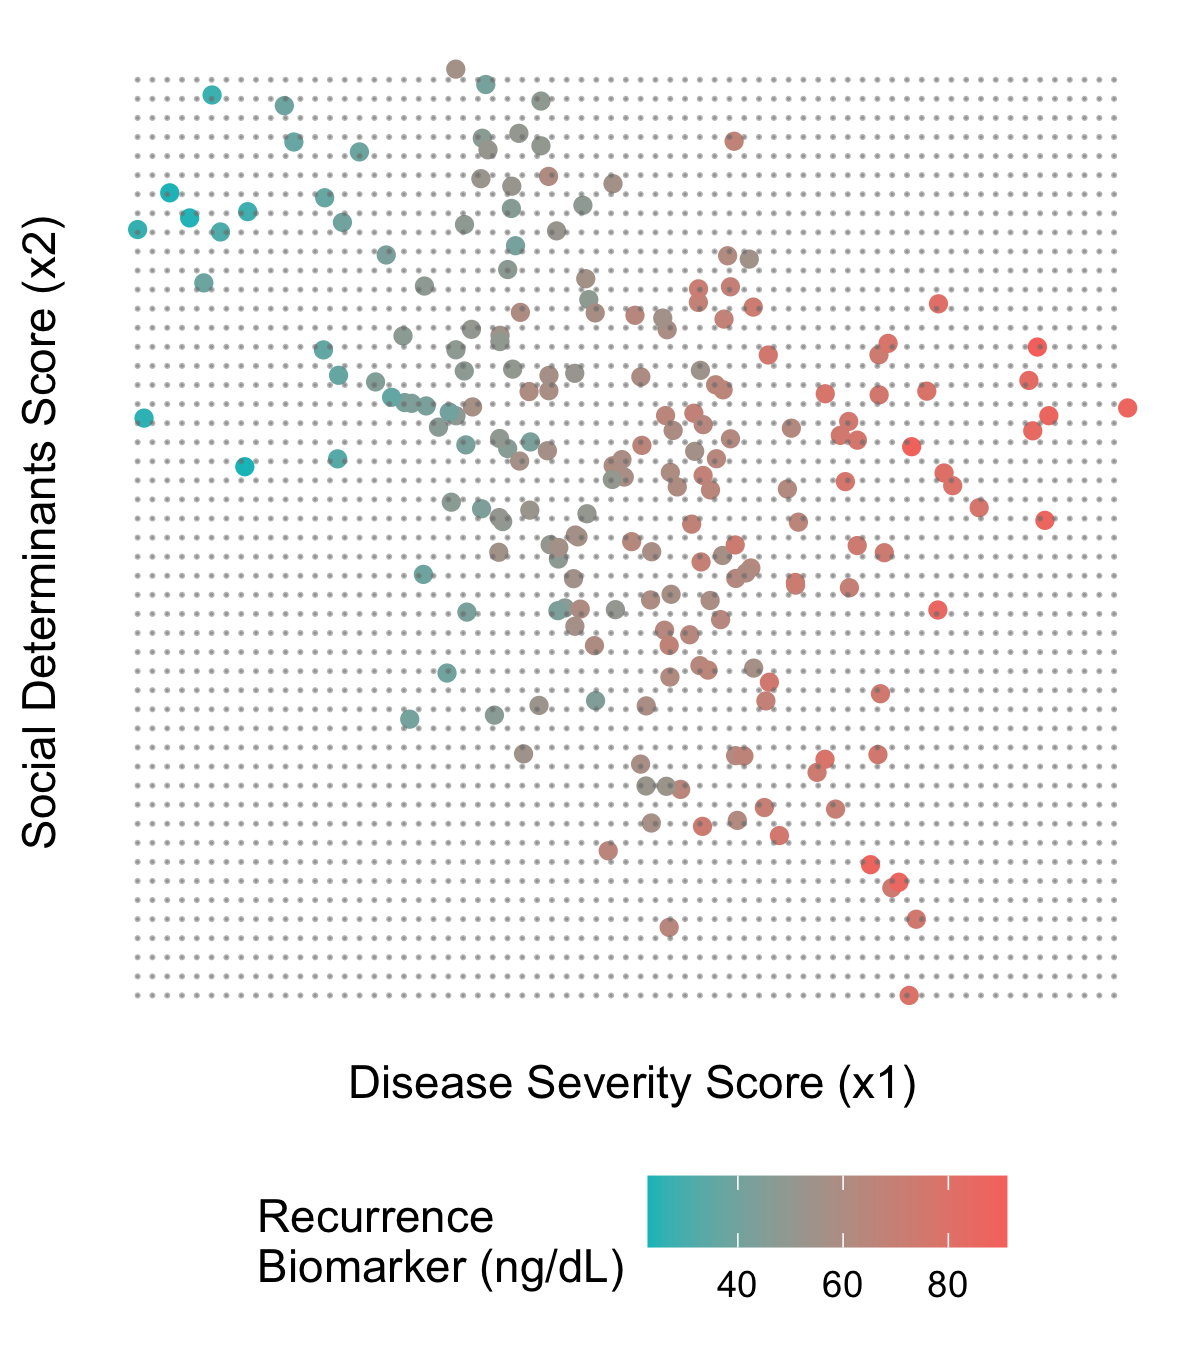
\includegraphics[width=0.65\textwidth]{img/esl-reg-just-data.png}
\end{center}

This is a plot of the data in a single plane. You can also view the data in 3D; here the color is redundant, since the height above the $x_1 \times x_2$ plane is represented separately.

\begin{center}
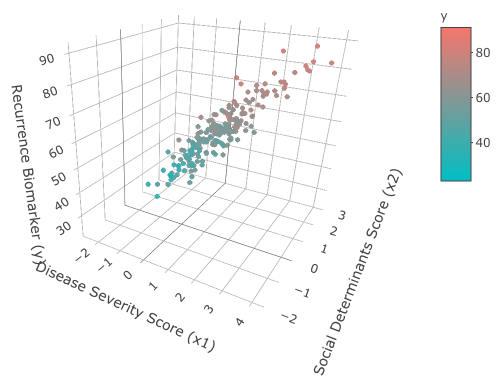
\includegraphics[width=0.7\textwidth]{img/esl-reg-3d-view-2.png}
\end{center}

%%%%%%%%%%%%%%%%%%%%%%%%%%%%%%%%%%%%%%%%%%%%%%%%%%%%%%%%%%%%%%%%%%%%%%%%%%%%%%%%%%%%%%

\section{Discussion Questions}

Think about the three algorithms we discussed in Chapter~\ref{chapter:classification}. Now think about our new task, which is to predict the \emph{numeric value} of the recurrence biomarker as a function of the two predictors, $x_1$ and $x_2$. 

\begin{enumerate}
\item Just looking at the two predictors, which one appears to more highly influence the value of the recurrence biomarker? Why?
\item How might you adapt KNN to deal with this problem?
\item How might you adapt a decision tree to deal with this problem?
\item How might you adapt logistic regression to deal with this problem? You'll have to ``break the algorithm'' a bit more this time.  
\item These plots are the regression equivalents of the plots we made in Chapter~\ref{chapter:classification}. They need to be 3D so you can see the geometry of the predictions more clearly. One contains predictions from KNN with $K=15$, one contains predictions from a decision tree, and one contains predictions from an algorithm called \textbf{linear regression}, which is a relative of logistic regression. Which algorithm goes with which plot?
\begin{center}
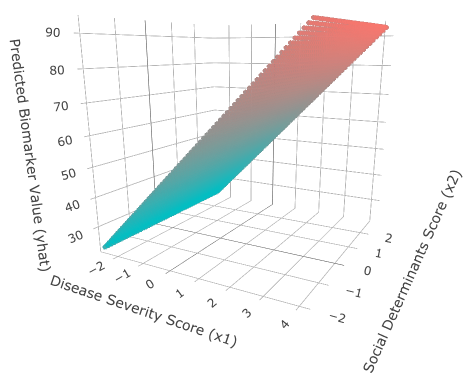
\includegraphics[width=0.7\textwidth]{img/esl-reg-3d-linear-small.png}
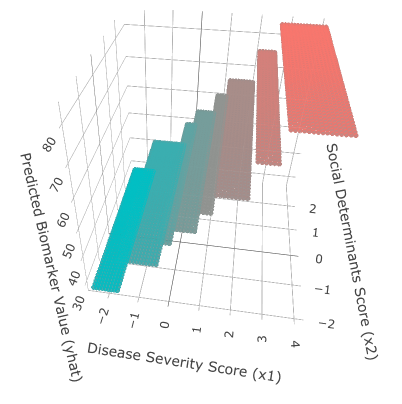
\includegraphics[width=0.6\textwidth]{img/esl-reg-3d-decision-tree-small.png}
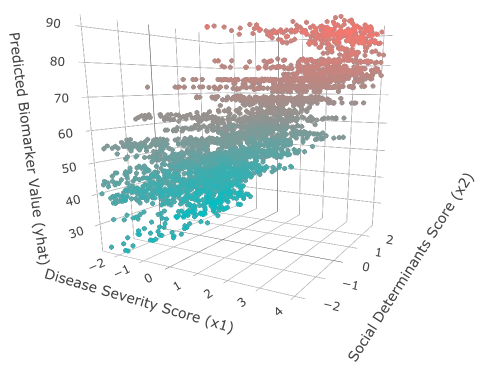
\includegraphics[width=0.7\textwidth]{img/esl-reg-3d-knn-15-small.png}
\end{center}
\item What are the advantages and disadvantages of each algorithm?
\end{enumerate}

